% \VignetteIndexEntry{hoa: An R Package Bundle for Higher Order Likelihood Inference}
% \VignetteDepends{survival}
% \VignetteKeyword{asymptotics}
% \VignetteKeyword{conditional inference}
% \VignetteKeyword{regression}

\documentclass[a4paper,11pt]{article}

\usepackage[round]{natbib}
\bibliographystyle{abbrvnat}

\def\R{{\sf R}}
\def\code{\texttt}

\title{\code{hoa}: An \R\ Package Bundle for Higher Order Likelihood Inference}
\author{by Alessandra R. Brazzale}
\date{\emph{Rnews}, \textbf{5/1} May 2005, pp.~20--27}

\usepackage{/Library/Frameworks/R.framework/Resources/share/texmf/Sweave}
\begin{document}

\maketitle

\section*{Introduction}
%
The likelihood function represents the basic ingredient of many commonly used statistical methods for estimation, testing and the calculation of confidence intervals.  In practice, much application of likelihood inference relies on first order asymptotic results such as the central limit theorem.  The approximations can, however, be rather poor if the sample size is small or, generally, when the average information available per parameter is limited.  Thanks to the great progress made over the past twenty-five years or so in the theory of likelihood inference, very accurate approximations to the distribution of statistics such as the likelihood ratio have been developed.  These not only provide modifications to well-established approaches, which result in more accurate inferences, but also give insight on when to rely upon first order methods.  We refer to these developments as \emph{higher order asymptotics}.  

One intriguing feature of the theory of higher order likelihood asymptotics is that relatively simple and familiar quantities play an essential role.  The higher order approximations discussed in this paper are for the significance function, which we will use to set confidence limits or to calculate the $p$-value associated with a particular hypothesis of interest.  We start with a concise overview of the approximations used in the remainder of the paper.  Our first example is an elementary one-parameter model where one can perform the calculations easily, chosen to illustrate the potential accuracy of the procedures.  Two more elaborate examples, an application of binary logistic regression and a nonlinear growth curve model, follow.  All examples are carried out using the \R\ code of the \code{hoa} package bundle. 


\section*{Basic ideas}
%
Assume we observed $n$ realizations $y_1, \ldots, y_n$ of independently distributed random variables $Y_1, \ldots, Y_n$ whose density function $f(y_i;\theta)$ depends on an unknown parameter $\theta$.  Let $\ell(\theta) = \sum_{i=1}^{n}\log f(y_i;\theta)$ denote the corresponding log likelihood and $\hat\theta = {\rm argmax}_\theta\ell(\theta)$ the maximum likelihood estimator.  In almost all applications the parameter $\theta$ is not scalar but a vector of length $d$.  Furthermore, we may re-express it as $\theta = (\psi,\lambda)$, where $\psi$ is the $d_0$-dimensional \emph{parameter of interest}, about which we wish to make inference, and $\lambda$ is a so-called \emph{nuisance parameter}, which is only included to make the model more realistic.  

Confidence intervals and $p$-values can be computed using the \emph{significance function} $p(\psi;\hat\psi) = {\rm Pr}(\hat\Psi \leq \hat\psi;\psi)$ which records the probability left of the observed ``data point'' $\hat\psi$ for varying values of the unknown parameter $\psi$ \citep{fraser:1991}.  Exact elimination of $\lambda$, however, is possible only in few special cases \citep[Sections~8.2 and 8.3]{severini:2000}.  A commonly used approach is to base inference about $\psi$ on the \emph{profile log likelihood} $\ell_{\rm p}(\psi) = \ell(\psi,\hat\lambda_\psi)$, which we obtain from the log likelihood function by replacing the nuisance parameter with its constrained estimate $\hat\lambda_\psi$ obtained by maximising $\ell(\theta) = \ell(\psi,\lambda)$ with respect to $\lambda$ for fixed $\psi$.  Let $j_{\rm p}(\psi)=-\partial^2\ell_{\rm p}(\psi)/\partial\psi\partial\psi^\top$ denote the observed information from the profile log likelihood.  Likelihood inference for scalar $\psi$ is typically based on the 
%
\begin{itemize}
\item Wald statistic, \ \ \ $w(\psi)  =  j_{\rm p}(\hat\psi)^{1/2}(\hat\psi - \psi)$; 
\item likelihood root, 
      \[
      r(\psi)  =  {\rm sign}(\hat\psi - \psi)\left[2\{\ell_{\rm p}(\hat\psi) -  \ell_{\rm p}(\psi)\}\right]^{1/2}; 
      \]
      or
\item score statistic, \ \ \ $s(\psi)  =  j_{\rm p}(\hat\psi)^{-1/2}d\ell_{\rm p}(\psi)/d\psi$.
\end{itemize}
%.
Under suitable regularity conditions on $f(y;\theta)$, all of these have asymptotic standard normal distribution up to the first order.  Using any of the above statistics we can approximate the significance function by $\Phi\{w(\psi)\}$, $\Phi\{r(\psi)\}$ or $\Phi\{s(\psi)\}$.  When $d_0 > 1$, we may use the quadratic forms of the Wald, likelihood root and score statistics whose finite sample distribution is $\chi^2_{d_0}$ with $d_0$ degrees of freedom up to the second order.  We refer the reader to Chapters~3 and 4 of \citet{severini:2000} for a review of first order likelihood inference.
 
Although it is common to treat $\ell_{\rm p}(\psi)$ as if it were an  ordinary log likelihood, first order approximations can give poor results, particularly if the dimension of $\lambda$ is high and the sample size small.  An important variant of the likelihood root is the \emph{modified likelihood root}
%
\begin{equation}
\label{eq:rstar}
r^*(\psi) = r(\psi) + \frac{1}{r(\psi)}\log\left\{q(\psi)/r(\psi)\right\},
\end{equation}
%
where $q(\psi)$ is a suitable correction term.  Expression~(\ref{eq:rstar}) is a higher order pivot whose finite sample distribution is standard normal up to the third order.  As it was the case for its first order counterpart $r$, the significance function is approximated by $\Phi\{r^*(\psi)\}$, and there is a version of $r^*$ for multidimensional $\psi$ \citep[Section~3.1]{skovgaard:2001}.  More details about the computation of the $q(\psi)$ correction term are given in the Appendix.    

It is sometimes useful to decompose the modified likelihood root as
%
\[
r^*(\psi) = r(\psi) + r_{\rm inf}(\psi) + r_{\rm np}(\psi),
\]
%
where $r_{\rm inf}$ is the \emph{information adjustment} and $r_{\rm np}$ is the \emph{nuisance parameter adjustment}.  The first term accounts for non normality of $r$, while the second compensates $r$ for the presence of the nuisance parameter $\lambda$.  \citet[Section~3]{pierce.peters:1992} discuss the behaviour of these two terms in the multiparameter exponential family context.  They find that while $r_{\rm np}$ is often appreciable, the information adjustment $r_{\rm inf}$ has typically a minor effect, provided the $\psi$-specific information $j_{\rm p}(\hat\psi)$ is not too small relative to the dimension of $\lambda$.  


\section*{A simple example}
%
Suppose that a sample $y_1, \ldots, y_n$ is available from the Cauchy density
%
\begin{equation}
\label{eq:Cauchy.density}
f(y;\theta) = \frac{1}{\pi\{1+(y-\theta)^2\}}.
\end{equation}
%
The maximum likelihood estimate $\hat\theta$ of the unknown location parameter $\theta$ is the value which maximises the log likelihood function
%
\[
\ell(\theta;y) = - \sum_{i=1}^{n}\log\{1+(y_i-\theta)^2\}.
\]
For $n=1$, we obtain the exact distribution of $\hat\theta = y$ from (\ref{eq:Cauchy.density}) as $F(\hat\theta;\theta) = F(y;\theta) = \pi^{-1}\arctan(y-\theta)$. 

\begin{figure}[htp]
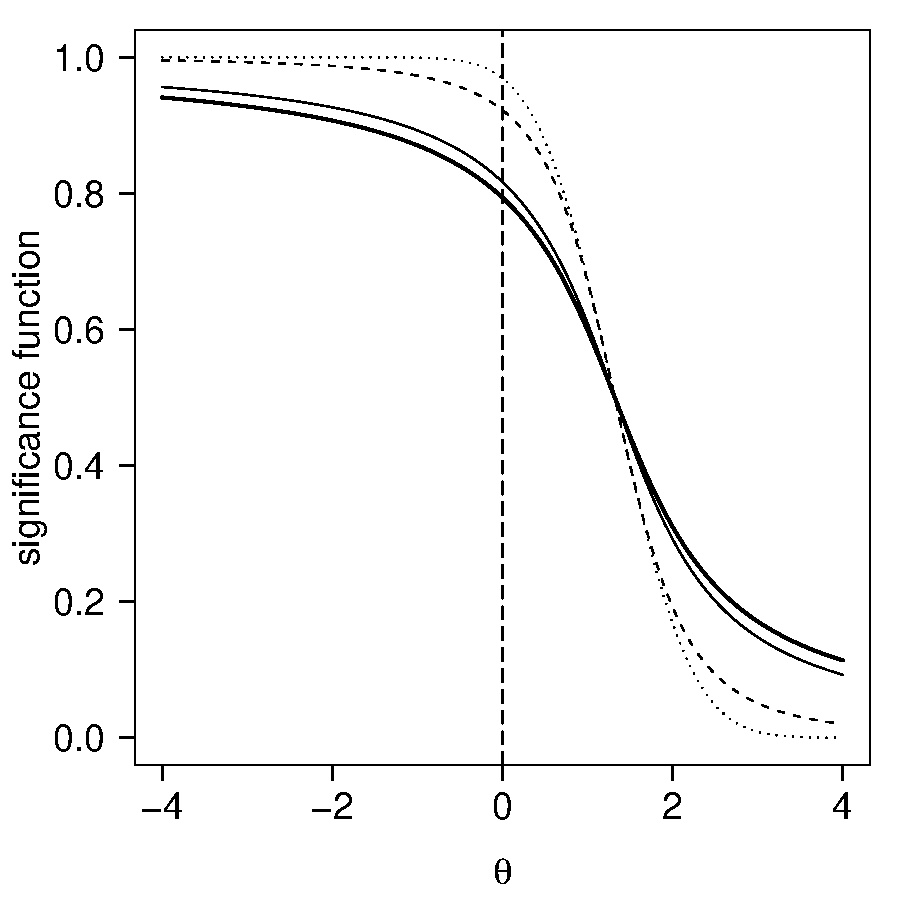
\includegraphics{Rnews-paper-001}
\caption{
Significance functions for the location parameter of a Cauchy distribution when $y = 1.32$: exact (bold), Wald pivot (dotted), $r$ (dashed) and $r^*$ (solid).  The vertical dashed line corresponds to the null hypothesis $\theta = 0$.}
\label{fig:signif.Cauchy}
\end{figure}

Assume that $y=1.32$ was observed.  In Figure~\ref{fig:signif.Cauchy} we compare the exact significance function $p(\theta;y) = {\rm Pr}(Y\leq y;\theta)$ (bold line) to the two first order approximations obtained from the Wald statistic 
%
\[
w(\theta) = \sqrt{2}(y-\theta),
\]
%
(dotted line), and from the likelihood root 
%
\[
r(\theta) = {\rm sign}(\hat\theta - \theta)\left[2\log\{1+(y-\theta)^2\}\right]^{1/2},
\]
%
(dashed line).  We also show the third order approximation $\Phi\{r^*(\theta)\}$ (solid line).  Since this is a location model and there is no nuisance parameter, the statistic $q(\theta)$ in (\ref{eq:rstar}) is the score statistic 
%
\[
s(\theta) = \sqrt{2}(y-\theta)/\{1+(y-\theta)^2\}
\]
%
(see formula~(\ref{eq:qreg}) in the Appendix).  The code used to generate Figure~\ref{fig:signif.Cauchy} is given below.

\begin{Schunk}
\begin{Sinput}
> wald.stat <- function(theta, y) {
+     sqrt(2) * (y - theta)
+ }
> lik.root <- function(theta, y) {
+     sign(y - theta) * sqrt(2 * log(1 + (y - theta)^2))
+ }
> score.stat <- function(theta, y) {
+     (sqrt(2) * (y - theta))/(1 + (y - theta)^2)
+ }
> rstar <- function(theta, y) {
+     lik.root(theta, y) + 1/lik.root(theta, y) * log(score.stat(theta, 
+         y)/lik.root(theta, y))
+ }
> theta.seq <- seq(-4, 4, length = 100)
> par(las = 1, mai = c(0.9, 0.9, 0.2, 0.2))
> plot(theta.seq, pcauchy(q = 1.32 - theta.seq), type = "l", lwd = 2, 
+     ylim = c(0, 1), xlab = expression(theta), ylab = "significance function", 
+     cex.lab = 1.5, cex.axis = 1.5)
> lines(theta.seq, pnorm(wald.stat(theta.seq, 1.32)), lty = "dotted")
> lines(theta.seq, pnorm(lik.root(theta.seq, 1.32)), lty = "dashed")
> lines(theta.seq, pnorm(rstar(theta.seq, 1.32)), lty = "solid")
> abline(v = 0, lty = "longdash")
\end{Sinput}
\end{Schunk}
%
The vertical dashed line corresponds to the null hypothesis that $\theta = 0$.  The exact $p$-value is 
%
\begin{Schunk}
\begin{Sinput}
> round(2 * (min(tp <- pt(1.32, df = 1), 1 - tp)), digits = 3)
\end{Sinput}
\begin{Soutput}
[1] 0.413
\end{Soutput}
\end{Schunk}
%
while the first and third order approximations yield 
%
\begin{Schunk}
\begin{Sinput}
> round(2 * (min(tp <- pnorm(wald.stat(0, 1.32)), 1 - tp)), digits = 3)
\end{Sinput}
\begin{Soutput}
[1] 0.062
\end{Soutput}
\begin{Sinput}
> round(2 * (min(tp <- pnorm(lik.root(0, 1.32)), 1 - tp)), digits = 3)
\end{Sinput}
\begin{Soutput}
[1] 0.155
\end{Soutput}
\begin{Sinput}
> round(2 * (min(tp <- pnorm(rstar(0, 1.32)), 1 - tp)), digits = 3)
\end{Sinput}
\begin{Soutput}
[1] 0.367
\end{Soutput}
\end{Schunk}
%
respectively for the Wald, likelihood root and modified likelihood root pivot.  The $r^*$ statistic is strikingly accurate, while the first order approximations are very poor.  This is surprising if we consider that the score function is not monotonic in $y$ and that only one observation is available.  

Suppose now that we observed a sample of size $n = 15$ from the Student t distribution with $3$ degrees of freedom.  It is no longer possible to derive the exact distribution of the maximum likelihood estimator $\hat\theta$, but we may use the code provided in the \code{marg} package of the \code{hoa} package bundle to compute the $p$-values for testing the significance of the location parameter.  

\begin{Schunk}
\begin{Sinput}
> library(marg)
\end{Sinput}
\begin{Soutput}
   Package "marg" 1.1-1 (2006-12-16) 
   Copyright (C) 2000-2006 A. R. Brazzale

This is free software, and you are welcome to redistribute
it and/or modify it under the terms of the GNU General
Public License published by the Free Software Foundation.
Package "marg" comes with ABSOLUTELY NO WARRANTY.

type `help(package="marg")' for summary information
\end{Soutput}
\begin{Sinput}
> set.seed(321)
> y <- rt(n = 15, df = 3)
> y.rsm <- rsm(y ~ 1, family = student(3))
> y.cond <- cond(y.rsm, offset = 1)
> summary(y.cond, test = 0)
\end{Sinput}
\begin{Soutput}
 Formula:  y ~ 1
 Family:  student
 Offset:  Intercept

          Estimate   Std. Error 
uncond.     -0.4208       0.3907
cond.       -0.4065       0.4313

Test statistics
---------------
 hypothesis : Intercept = 0 
                           statistic  tail prob.
Wald pivot                   -1.0770      0.1408
Wald pivot (cond.)           -0.9426      0.1729
Likelihood root              -1.0250      0.1528
Modified likelihood root     -0.9277      0.1768
                            
"q" correction term: -0.9277

Diagnostics:
----------- 
   INF     NP 
0.2057 0.3291 

 Approximation based on 20 points
\end{Soutput}
\end{Schunk}

The previous set of instructions yields the $p$-values $0.282$ (Wald), $0.306$ ($r$) and $0.354$ ($r^*$).  The difference between first order and higher order approximations is slightly smaller than it was the case before.  For this particular model a sample size of $n=15$ still does not provide enough information on the scalar parameter $\theta$ to wipe out completely the effect of higher order corrections. 


\section*{Higher order asymptotics in \R}
%
\code{hoa} is an \R\ package bundle which implements higher order inference for three widely used model classes: logistic regression, linear non normal models and nonlinear regression with possibly non homogeneous variance.  The corresponding code is organised in three packages, namely \code{cond}, \code{marg} and \code{nlreg}.  We already saw a (very elementary) application of the \code{marg} code.  The two examples which follow will give a glimpse of the use of the routines in \code{cond} and \code{nlreg}.  Attention is restricted to the calculation of $p$-values and confidence intervals, although several routines for accurate point estimation and model checking are also available.  The \code{hoa} bundle includes a fourth package, called \code{sampling}, which we will not discuss here.  It implements a Metropolis-Hastings sampler which can be used to simulate from the conditional distribution of the higher order statistics considered in \code{marg}.  

The \code{hoa} package bundle is be available on CRAN.  More examples of applications, and generally of the use of likelihood asymptotics, are given in \citet{brazzale.davison.reid:2006}.

\section*{Example 1: Binary data}
%
\citet{collet:1998} gives a set of binary data on the presence of a sore throat in a sample of $35$ patients undergoing surgery during which either of two devices was used to secure the airway.  
%
\begin{Schunk}
\begin{Sinput}
> library(cond)
\end{Sinput}
\begin{Soutput}
   Package "cond" 1.1-1 (2006-12-16) 
   Copyright (C) 2000-2006 A. R. Brazzale

This is free software, and you are welcome to redistribute
it and/or modify it under the terms of the GNU General
Public License published by the Free Software Foundation.
Package "cond" comes with ABSOLUTELY NO WARRANTY.

type `help(package="cond")' for summary information
\end{Soutput}
\begin{Sinput}
> head(airway, n = 3)
\end{Sinput}
\begin{Soutput}
  response age sex lubricant duration type
1        0  48   1         0       45    0
2        0  48   1         0       15    0
3        1  39   0         1       40    0
\end{Soutput}
\end{Schunk}
%
In addition to the variable of interest, device \code{type}  (1=tracheal tube or 0=laryngeal mask), there are four further explanatory variables: the \code{age} of the patient in years, an indicator variable for \code{sex} (1=male, 0=female), an indicator variable for \code{lubricant} use (1=yes, 0=no) and the \code{duration} of the surgery in minutes.  The observations form the data frame \code{airway} which is part of the \code{hoa} bundle. 

A natural starting point for the analysis is a logistic regression model with success probability of the form
%
\[
{\rm Pr}(Y=1;\beta) = \frac{\exp(x^\top\beta)}{1+\exp(x^\top\beta)},
\]
%
where $x$ represents the explanatory variables associated with the binary \code{response} $Y$ (1=sore throat and 0=no sore throat).  The following set of instructions fits this model to the data with all five explanatory variables included.  
%
\begin{Schunk}
\begin{Sinput}
> airway.glm <- glm(formula(airway), family = binomial, data = airway)
> summary(airway.glm)
\end{Sinput}
\begin{Soutput}
Call:
glm(formula = formula(airway), family = binomial, data = airway)

Deviance Residuals: 
    Min       1Q   Median       3Q      Max  
-2.1888  -0.5633   0.3029   0.7444   1.5954  

Coefficients:
            Estimate Std. Error z value Pr(>|z|)  
(Intercept) -2.75035    2.08914  -1.316   0.1880  
age          0.02245    0.03763   0.597   0.5507  
sex1         0.32076    1.01901   0.315   0.7529  
lubricant1   0.08448    0.97365   0.087   0.9309  
duration     0.07183    0.02956   2.430   0.0151 *
type1       -1.62968    0.94737  -1.720   0.0854 .
---
Signif. codes:  0 '***' 0.001 '**' 0.01 '*' 0.05 '.' 0.1 ' ' 1 

(Dispersion parameter for binomial family taken to be 1)

    Null deviance: 46.180  on 34  degrees of freedom
Residual deviance: 29.477  on 29  degrees of freedom
AIC: 41.477

Number of Fisher Scoring iterations: 5
\end{Soutput}
\end{Schunk}
%
The coefficient of device \code{type} is only marginally significant.  

As in the previous example we may wonder whether the sample size is large enough to allow us to rely upon first order inference.  For the airway data we have $n=35$ and $p=5$, so we might expect higher order corrections to the usual approximations to have little effect.  We can check this using the routines in the \code{cond} package.
%
\begin{Schunk}
\begin{Sinput}
> airway.cond <- cond(airway.glm, offset = type1)
> summary(airway.cond)
\end{Sinput}
\begin{Soutput}
 Formula:  response ~ age + sex + lubricant + duration + type
 Family:  binomial
 Offset:  type1

          Estimate   Std. Error 
uncond.      -1.630       0.9474
cond.        -1.394       0.8466

Confidence intervals
--------------------
 level = 95 %
                                         lower two-sided  upper
Wald pivot                              -3.486           0.2271
Wald pivot (cond. MLE)                  -3.053           0.2655
Likelihood root                         -3.682           0.1542
Modified likelihood root                -3.130           0.2558
Modified likelihood root (cont. corr.)  -3.592           0.5649

Diagnostics:
----------- 
    INF      NP 
0.05855 0.51426 

 Approximation based on 20 points
\end{Soutput}
\begin{Sinput}
> plot(airway.cond, which = 4)
\end{Sinput}
\end{Schunk}
%
As our model is a canonical exponential family, the correction term $q(\psi)$ in (\ref{eq:rstar}) involves the Wald statistic $w(\psi)$ plus parts of the observed information matrix (see formula~(\ref{eq:qexp}) in the Appendix).  The 95\% confidence intervals obtained from the Wald pivot and from the likelihood root are respectively $(-3.486, 0.227)$ and $(-3.682,  0.154)$.  The third order statistic $r^*$ yields a 95\% confidence interval of $(-3.130, 0.256)$.  First and third order results are rather different, especially with respect to the lower bound.  Figure~\ref{fig:pivot.airway} plots the profiles of the first and third order pivots $w(\psi)$ (dashed line), $r(\psi)$ (solid line) and $r^*(\psi)$ (bold line).  The correction term $q(\psi)$ is particularly significant for values of $\psi$ belonging to the lower half of the confidence interval.  The nuisance parameter correction is $r_{\rm np}=0.51$, while $r_{\rm inf}=0.059$
is about ten times smaller.

\begin{figure}[tph]
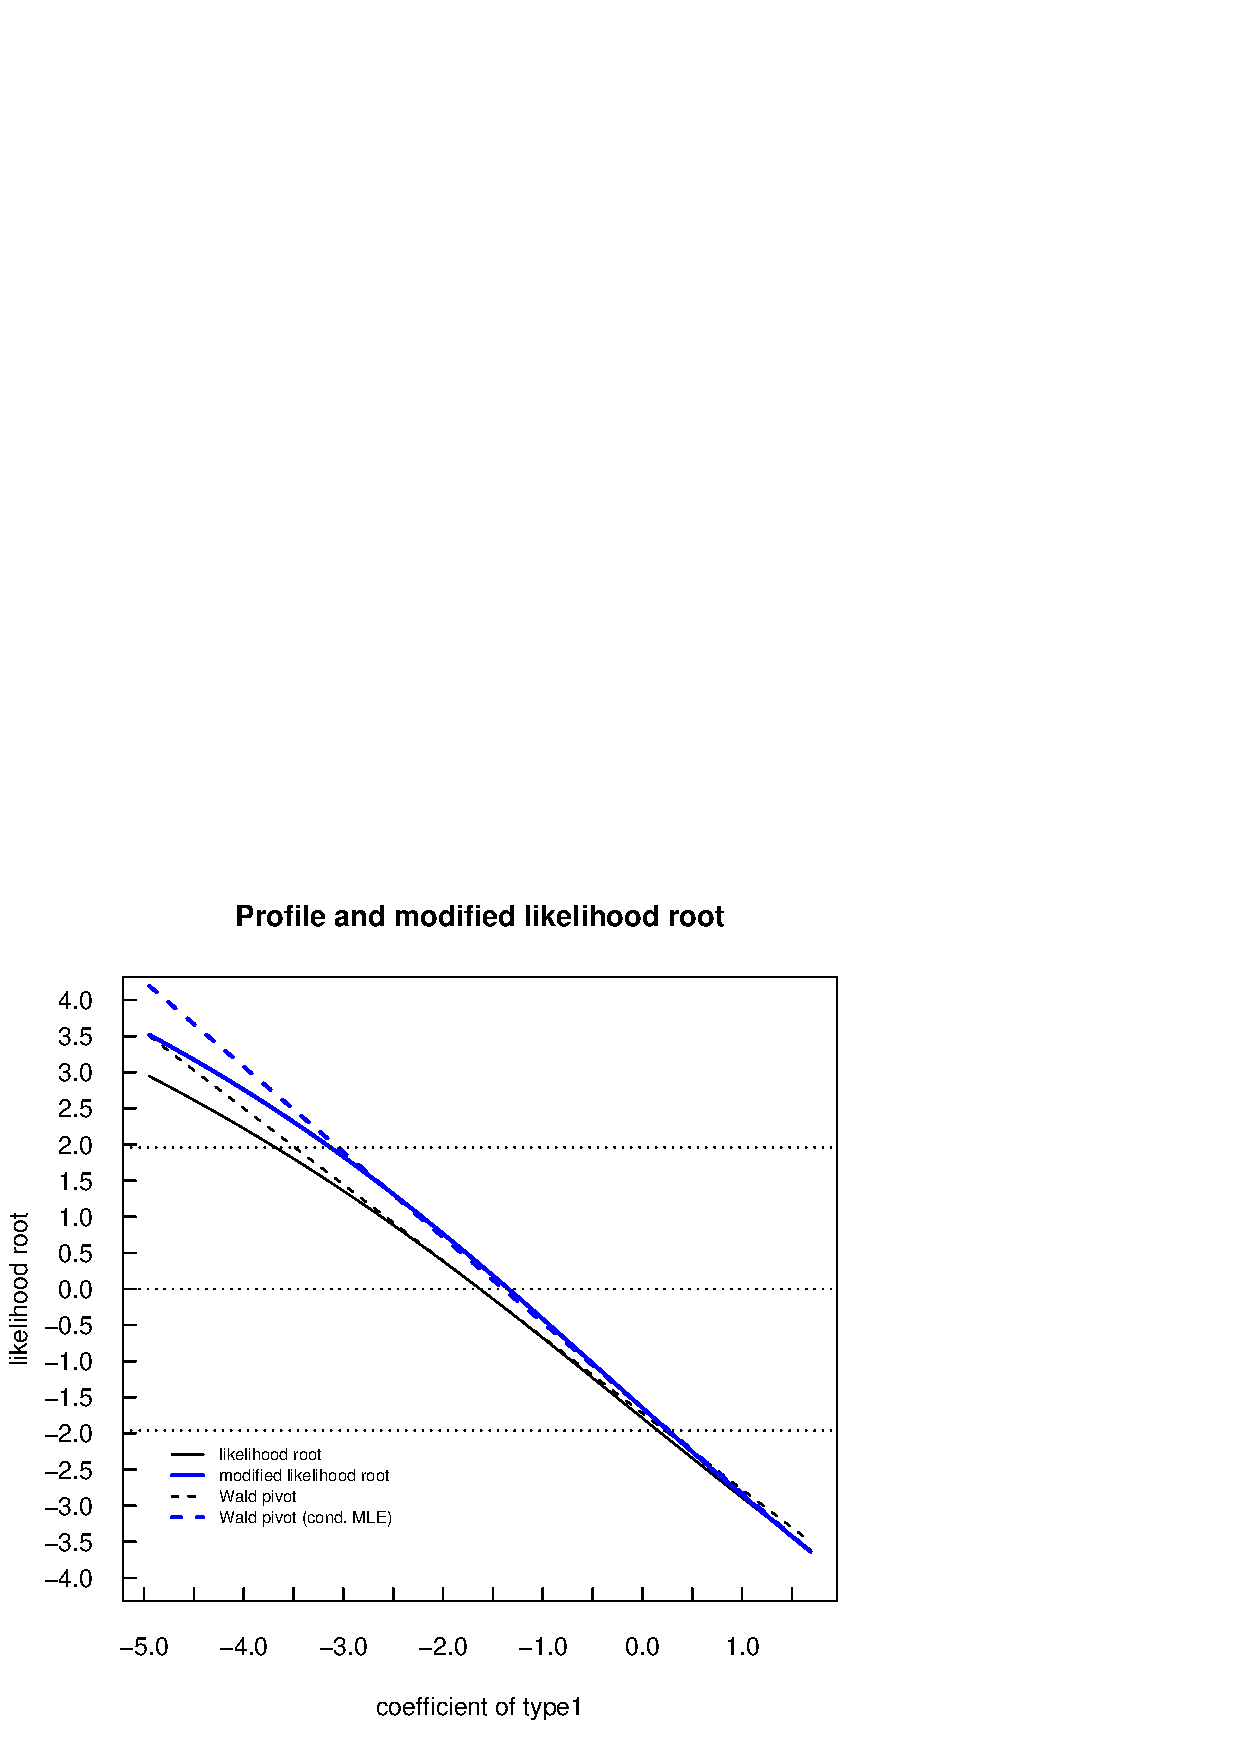
\includegraphics{Rnews-paper-009}
\caption{
\code{airway} data analysis: profile plots of the pivots $w(\psi)$ (dashed line), $r(\psi)$ (solid line) and $r^*(\psi)$ (bold line), where $\psi$ is the coefficient of the covariate device \code{type}.}
\label{fig:pivot.airway}
\end{figure}


\section*{Example 2: Nonlinear regression}
%
A simple illustration of nonlinear regression is Example~7.7 of \citet{davison.hinkley:1997}, which refers to the \code{calcium} data of package \code{boot}.  This data set records the calcium uptake (in nmoles/mg) of cells $y$ as a function of time $x$ (in minutes), after being suspended in a solution of radioactive calcium.  
%
\begin{Schunk}
\begin{Sinput}
> library(boot)
> head(calcium, n = 3)
\end{Sinput}
\begin{Soutput}
  time      cal
1 0.45  0.34170
2 0.45 -0.00438
3 0.45  0.82531
\end{Soutput}
\end{Schunk}
%
The variables \code{cal} and \code{time} represent respectively the calcium uptake and suspension time.  There are 27 observations in all.  The model is 
%
\begin{equation}
\label{eq:calcium.mod}
y_i = \beta_0\{1-\exp(-\beta_1x_i)\} + \sigma_i\varepsilon_i,
\end{equation}
%
where $\beta_0$ and $\beta_1$ are unknown regression coefficients and the error term $\varepsilon_i \sim N(0,1)$ is standard normal.  We complete the definition of model~(\ref{eq:calcium.mod}) by allowing the response variance $\sigma^2_i = \sigma^2(1+x_i)^\gamma$ to depend nonlinearly on the time covariate through the two variance parameters $\gamma$ and $\sigma^2$.  

Model~(\ref{eq:calcium.mod}) is fitted by maximum likelihood using the \code{nlreg} routine of package \code{nlreg}.
%
\begin{Schunk}
\begin{Sinput}
> library(nlreg)
\end{Sinput}
\begin{Soutput}
   Package "nlreg" 1.1-1 (2006-12-16) 
   Copyright (C) 2000-2006 R. Bellio & A. R. Brazzale

This is free software, and you are welcome to redistribute
it and/or modify it under the terms of the GNU General
Public License published by the Free Software Foundation.
Package "nlreg" comes with ABSOLUTELY NO WARRANTY.

type `help(package="nlreg")' for summary information
\end{Soutput}
\begin{Sinput}
> calcium.nl <- nlreg(cal ~ b0 * (1 - exp(-b1 * time)), weights = ~(1 + 
+     time)^g, data = calcium, start = c(b0 = 4, b1 = 0.1, g = 0))
> summary(calcium.nl)
\end{Sinput}
\begin{Soutput}
differentiating mean function -- may take a while
differentiating variance function -- may take a while
Call: 
nlreg(formula = cal ~ b0 * (1 - exp(-b1 * time)), weights = ~(1 + 
    time)^g, data = calcium, start = c(b0 = 4, b1 = 0.1, g = 0))

Regression coefficients:
   Estimate Std. Error z value Pr(>|z|)    
b0  4.31699    0.32274   13.38  < 2e-16 ***
b1  0.20746    0.03589    5.78 7.47e-09 ***
---
Signif. codes:  0 '***' 0.001 '**' 0.01 '*' 0.05 '.' 0.1 ' ' 1 

Variance parameters:
     Estimate Std. Error
g      0.5364     0.3196
logs  -2.3426     0.6338

No interest parameter

Total number of observations: 27
Total number of parameters: 4
-2*Log Likelihood 39.31 

Algorithm converged in 3 iterations
\end{Soutput}
\end{Schunk}
%
This yields $\hat\beta_0 = 4.317$ (s.e.\ $0.323$), $\hat\beta_1 = 0.207$ (s.e.\ $0.036$), $\hat\gamma = 0.536$ (s.e.\ $0.320$), and $\log\hat\sigma^2 = -2.343$ (s.e.\ $0.634$).  Note that the baseline variance $\sigma^2$ is fitted on the logarithmic scale.  This does not affect inference based on the $r$ and $r^*$ statistics, which are parametrisation invariant, and ensures positive values for $\sigma^2$ when the Wald statistic is used.  The \code{profile} method of the \code{nlreg} package can be used to set various first and higher order 95\% confidence intervals for the variance parameter $\gamma$.
%
\begin{Schunk}
\begin{Sinput}
> calcium.prof <- profile(calcium.nl, offset = g)
\end{Sinput}
\begin{Soutput}
differentiating mean function -- may take a while
differentiating variance function -- may take a while
\end{Soutput}
\begin{Sinput}
> summary(calcium.prof)
\end{Sinput}
\begin{Soutput}
 Two-sided confidence intervals for g 
                  lower upper
r* - Fr (0.95) -0.14340 1.191
r* - Sk (0.95) -0.14320 1.190
r (0.95)       -0.12441 1.154
Wald (0.95)    -0.08991 1.163
                             
  Estimate Std. Error
g   0.5364     0.3196

14 points calculated exactly
50 points used in spline interpolation

INF (Sk): 0.05793
INF (Fr): 0.06984
NP (Sk): 0.152
NP (Fr): 0.141 
\end{Soutput}
\end{Schunk}
%
A difficulty we had not to face in the previous two examples is that it is no longer possible to calculate the correction term in (\ref{eq:rstar}) exactly.  The \code{profile} function implements two slightly different versions of the higher order pivot $r^*$ which we obtain by using the two approximations of $q(\psi)$ discussed in the Appendix.  The four statistics agree in letting us question the heterogeneity of the response variance.  
 
\citet[p.~356]{davison.hinkley:1997} consider not only inference on the nonlinear mean function, but also on other aspects of the model such as the ``proportion of maximum'', $\pi = 1-\exp(-\beta_1x)$.  For $x = 15$ minutes they give the estimate $\hat\pi = 0.956$ and the associated 95\% bootstrap confidence interval $(0.83,0.98)$.  We may obtain the corresponding first and higher order likelihood  analogues by reparametrizing the mean response curve into $(\pi,\beta_0)$ and re-running the whole analysis.  This time we assume that the response variance is homogeneous.  
%
\begin{Schunk}
\begin{Sinput}
> calcium.nl <- nlreg(cal ~ b0 * (1 - exp(-log(1 + exp(psi)) * 
+     time/15)), data = calcium, start = c(b0 = 4.3, psi = 2))
> calcium.prof <- profile(calcium.nl, offset = psi)
\end{Sinput}
\begin{Soutput}
differentiating mean function -- may take a while
differentiating variance function -- may take a while
\end{Soutput}
\begin{Sinput}
> calcium.sum <- summary(calcium.prof)
> exp(calcium.sum$CI)/(1 + exp(calcium.sum$CI))
\end{Sinput}
\begin{Soutput}
                   lower     upper
r* - Fr (0.95) 0.8748267 0.9897534
r* - Sk (0.95) 0.8715956 0.9892019
r (0.95)       0.8777616 0.9882782
Wald (0.95)    0.8728598 0.9857717
\end{Soutput}
\end{Schunk}
%
Because of the constraint that $\pi$ must lie in the interval $(0,1)$, we actually fit the model for $\psi = \log\{\pi/(1-\pi)\}$ and back-transform to the original scale by $\pi = \exp(\psi)/\{1+\exp(\psi)\}$.  This yields the intervals $(0.87,0.99)$ and $(0.88,0.99)$ for respectively the Wald and likelihood root statistics and $(0.87,0.99)$ for both versions of $r^*$, which is in agreement with the bootstrap simulation.  

The \code{profile} method of the \code{nlreg} package provides also all elements needed to display graphically a fitted nonlinear model.
%
\begin{Schunk}
\begin{Sinput}
> calcium.prof <- profile(calcium.nl)
\end{Sinput}
\begin{Soutput}
long calculation --- may take a while

differentiating mean function -- may take a while
differentiating variance function -- may take a while
\end{Soutput}
\begin{Sinput}
> par(las = 1, mai = c(0.5, 0.5, 0.2, 0.2))
> contour(calcium.prof, alpha = 0.05, cl1 = "black", cl2 = "black", 
+     lwd2 = 2)
\end{Sinput}
\begin{Soutput}
Higher order method used: Skovgaard's r*
\end{Soutput}
\end{Schunk}
%
The result is Figure~\ref{fig:contour.calcium}.  The \code{contour} method of the \code{nlreg} package represents, in fact, an enhanced version of the original algorithm by \citet[Chapter~6]{bates.watts:1988}, to which we refer the reader for the interpretation of these plots.  The dashed, solid and bold lines represent respectively the Wald pivot, the likelihood root $r$ and Skovgaard's (1996) approximation to the $r^*$ statistic (see the Appendix).  The bivariate contour plots in the lower triangle are plotted on the original scale, whereas the ones in the upper triangle are on the $r$ scale.  Figure~\ref{fig:contour.calcium} highlights different aspects of the model fit.  First, the maximum likelihood estimate of $\log\sigma^2$ is biased downwards, which we can tell from the fact the corresponding $r^*$ profile is shifted to the right of $r$.  Otherwise, there does not seem to be a huge difference between first and higher order methods as the corresponding profiles and contours are not too different.  The finite sample estimates of $\beta_0$ and $\psi$ are strongly correlated, while they are almost independent of $\log\hat\sigma^2$.  The contours of $r(\psi)$ and $r^*(\psi)$ are close to elliptic which indicates that the log likelihood function is not too far from being quadratic.  A further indication for a small curvature effect due to parametrisation is that the contours on the original and on the $r$ scale look similar. 

\begin{figure}[tp]
\begin{Schunk}
\begin{Soutput}
Higher order method used: Skovgaard's r*
\end{Soutput}
\end{Schunk}
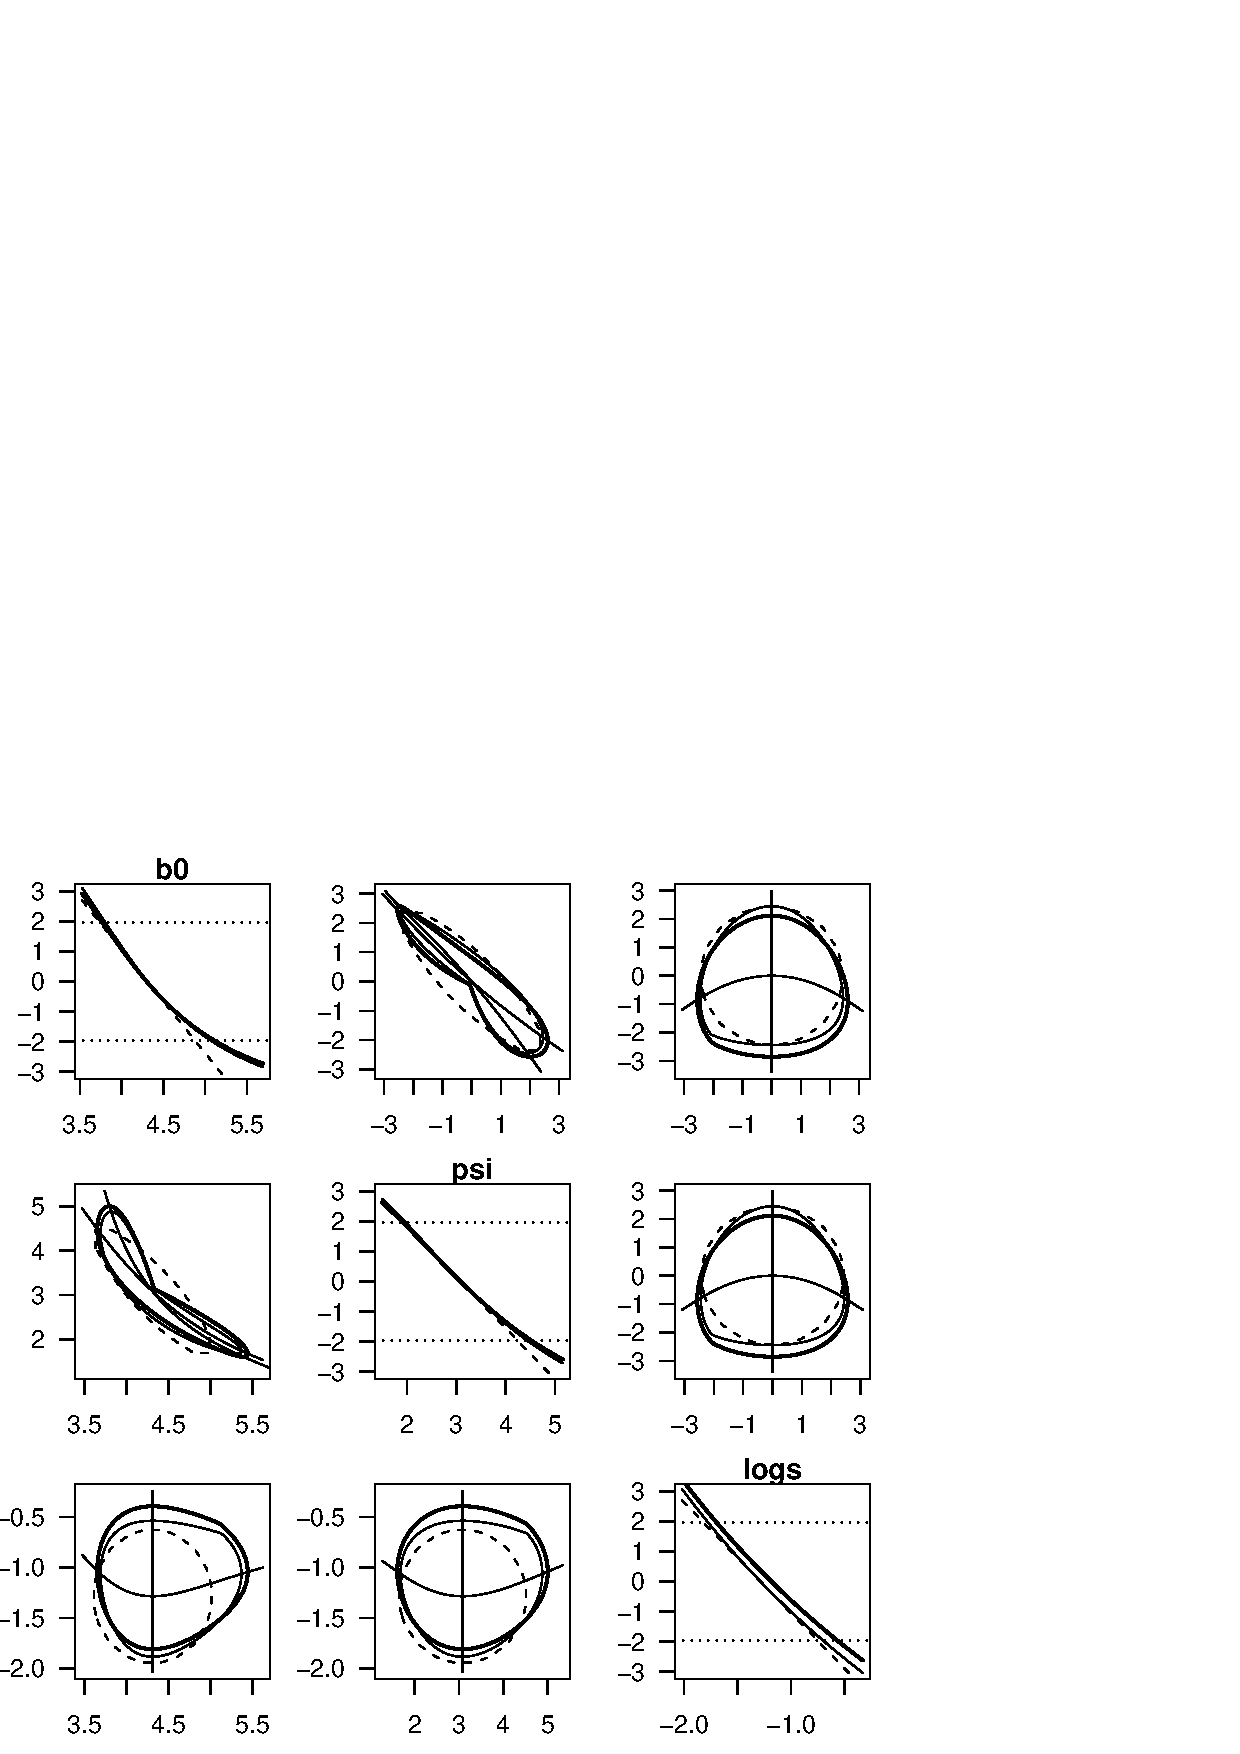
\includegraphics{Rnews-paper-015}
\caption{
\code{calcium} uptake data analysis: profile plots and profile pair sketches for the parameters $\beta_0$, $\psi$ and $\log\sigma^2$ using the Wald statistic (dashed), the likelihood root $r$ (solid) and Skovgaard's (1996) approximation to $r^*$ (bold).}
\label{fig:contour.calcium}
\end{figure}


\section*{Acknowledgments}
%
I am in debt with Ruggero Bellio, Anthony Davison and Nancy Reid for the many helpful discussions on and around higher order likelihood asymptotics.  I would like to thank two anonymous referees whose suggestions and comments helped improving a previous version of this paper.  


\appendix


\section*{Appendix: $q(\psi)$ correction term}
%  
In this appendix we give the general expression of the correction term $q(\psi)$ in (\ref{eq:rstar}) and the explicit formulae for two special model classes, that is, linear exponential families and regression-scale models.  We will furthermore discuss two ways of approximating $q(\psi)$ in case we cannot calculate it explicitly. 


\subsection*{Basic expression}
%
Let $\ell(\theta)=\ell(\psi,\lambda)$ be the log likelihood function, $\hat\theta = (\hat\psi,\hat\lambda)$ the maximum likelihood estimator of the $d$-dimensional parameter $\theta = (\psi,\lambda)$, and $j(\theta) = -\partial^2\ell(\theta)/\partial\theta\partial\theta^\top$ the $d\times d$ observed information matrix.  Denote $\hat\lambda_\psi$ the constrained maximum likelihood estimator of the nuisance parameter $\lambda$ given the value of the scalar parameter of interest $\psi$.  Write $j_{\lambda\lambda}(\theta)$ the corner of $j(\theta) = j(\psi,\lambda)$ which corresponds to $\lambda$, and $\hat\theta_\psi = (\psi, \hat\lambda_\psi)$.  

The basic expression for $q(\psi)$ is
%
\begin{equation}
\label{eq:qterm}
q(\psi) = \frac{| \ell_{;\hat\theta}(\hat\theta) - \ell_{;\hat\theta}(\hat\theta_\psi) 
              \ \ \ 
              \ell_{\lambda^\top;\hat\theta}(\hat\theta_\psi) |}
               {\left\{| j_{\lambda\lambda}(\hat\theta_\psi) | | j(\hat\theta) |\right\}^{1/2}},
\end{equation}
%
where $|\cdot|$ indicates determinant \citep[Section~7.4.1]{severini:2000}.  The $d\times d$ matrix appearing in the numerator of $q(\psi)$ consists of a column vector formed using so-called \emph{sample space derivatives}
%
\[
\ell_{;\hat\theta}(\theta) = \frac{\partial\ell(\theta;\hat\theta|a)}{\partial\hat\theta},
\]
%
and a $d\times (d-1)$ matrix of \emph{mixed derivatives}
%
\[
\ell_{\lambda^\top;\hat\theta} = \frac{\partial^2\ell(\psi,\lambda;\hat\theta|a)}{\partial\lambda^\top\partial\hat\theta}.
\]
%
The former are defined as the derivatives of the log likelihood function $\ell(\psi,\lambda;\hat\theta|a)$ with respect to the maximum likelihood estimator $\hat\theta$; mixed derivatives furthermore involve differentiation with respect to the whole parameter $\theta$ or parts of it \citep[Section~6.2.1]{severini:2000}.  Note that to do so, the data vector has to be re-expressed as $y = (\hat\theta, a)$, where $a$ represents the observed value of an ancillary statistic upon which we condition.     


\subsection*{Approximations}
%
Exact computation of the sample space derivatives involved in expression~(\ref{eq:qterm}) requires that we are able to write the data vector $y$ as a function of the maximum likelihood estimator $\hat\theta$ and of an ancillary statistic $a$.  This is, with few exceptions, only feasible for linear exponential families and transformation models, in which cases the $q(\psi)$ term involves familiar likelihood quantities.  If the reference model is a full rank exponential family with $\psi$ and $\lambda$ taken as canonical parameters, the correction term 
%
\begin{equation}
\label{eq:qexp}
q(\psi) = w(\psi) \left\{ 
          |j_{\lambda\lambda}(\hat\theta)|/|j_{\lambda\lambda}(\hat\theta_\psi)| \right\}^{1/2}
\end{equation}
%
depends upon the Wald statistic.  In case of a regression-scale model, that is, of a linear regression model with non necessarily normal errors,
%
\begin{equation}
\label{eq:qreg}
q(\psi) = s(\psi)  
          \left\{ |j_{\lambda\lambda}(\hat\theta_\psi)|/|j_{\lambda\lambda}(\hat\theta)| \right\}^{1/2}
\end{equation} 
%
involves the score statistic.  Here, $\psi$ is linear in $(\beta,\sigma)$ and the nuisance parameter $\lambda$ is taken linear in $\beta$ and $\xi = \log\sigma$, where $\beta$ and $\sigma$ represent respectively the regression coefficients and the scale parameter.

In general, the calculation of the sample space derivatives $\ell_{;\hat\theta}(\theta)$ and mixed derivatives $\ell_{\lambda^\top;\hat\theta}(\theta)$ may be difficult or impossible.  To deal with this difficulty, several approximations were proposed.  For a comprehensive review we refer the reader to Section~6.7 of \citet{severini:2000}.  Here we will mention two of them.  A first approximation, due to \citet{fraser.reid.wu:1999}, is based upon the idea that in order to differentiate the likelihood function $\ell(\theta;\hat\theta|a)$ on the surface in the $n$-dimensional sample space defined by conditioning on $a$ we need not know exactly the transformation from $y$ to $(\hat\theta,a)$, but only the $d$ vectors which are tangent to this surface \citep[Section~6.7.2]{severini:2000}.  \citet{skovgaard:1996} on the other hand suggests to approximate the sample space and mixed derivatives by suitable covariances of the log likelihood and of the score vector \citep[Section~6.7.3]{severini:2000}.  While the first approximation maintains the third order accuracy of $r^*$, we lose one degree when following Skovgaard's (1996) approach.  See Sections~7.5.3 and 7.5.4 of \citet{severini:2000} for the details.  


\subsection*{The \code{hoa} package}
%
The expressions of $q(\psi)$ implemented in the \code{hoa} package bundle are: i) (\ref{eq:qexp}) and (\ref{eq:qreg}) for respectively the \code{cond} and \code{marg} packages (logistic and linear non normal regression), and ii) the two approximations discussed above for the \code{nlreg} package (nonlinear heteroscedastic regression).  The formulae are given in \citet{brazzale.davison.reid:2006}.  The \code{nlreg} package also implements Skovgaard's (2001, Section~3.1)
\nocite{skovgaard:2001} multiparameter extension of the modified likelihood root.  The implementation of the \code{cond} and \code{nlreg} packages is discussed in \citet{brazzale:1999} and \citet{bellio.brazzale:2003}.


\begin{thebibliography}{10}
\expandafter\ifx\csname natexlab\endcsname\relax\def\natexlab#1{#1}\fi
\expandafter\ifx\csname url\endcsname\relax
  \def\url#1{{\tt #1}}\fi

\bibitem[Bates and Watts(1988)]{bates.watts:1988}
D.~M.~Bates and D.~G.~Watts.
\newblock {\em Nonlinear Regression Analysis and Its Applications}.
\newblock Wiley, New York, 1988.

\bibitem[Bellio and Brazzale(2003)]{bellio.brazzale:2003}
R.~Bellio and A.~R.~Brazzale.
\newblock Higher-order asymptotics unleashed: Software design for nonlinear heteroscedastic models.
\newblock {\em Journal of Computational and Graphical Statistics}, 12:\penalty0 682--697, 2003.

\bibitem[Brazzale(1999)]{brazzale:1999}
A.~R.~Brazzale.
\newblock Approximate conditional inference in logistic and loglinear models.
\newblock {\em Journal of Computational and Graphical Statistics}, 8:\penalty0 653--661, 1999.

\bibitem[Brazzale et~al.(to appear)Brazzale, Davison, and
  Reid]{brazzale.davison.reid:2006}
A.~R.~Brazzale, A.~C.~Davison, and N.~Reid.
\newblock {\em Applied Asymptotics}.
\newblock Cambridge University Press, Cambridge, to appear.

\bibitem[Collet(1998)]{collet:1998}
D.~Collet.
\newblock Binary data.
\newblock In P.~Armitage and T.~Colton, editors, {\em Encyclopedia of
  Biostatistics}. John Wiley \& Sons, Chichester, 1998.

\bibitem[Davison and Hinkley(1997)]{davison.hinkley:1997}
A.~C.~Davison and D.~V.~Hinkley.
\newblock {\em Bootstrap Methods and Their Application}.
\newblock Cambridge University Press, Cambridge, 1997.

\bibitem[Fraser(1991)]{fraser:1991}
D.~A.~S. Fraser.
\newblock Statistical inference: Likelihood to significance.
\newblock {\em Journal of the American Statistical Association}, 86:\penalty0
  258--265, 1991.

\bibitem[Fraser et~al.(1999)Fraser, Reid, and Wu]{fraser.reid.wu:1999}
D.~A.~S.~Fraser, N.~Reid, and J.~Wu.
\newblock A simple general formula for tail probabilities for frequentist and
  Bayesian inference.
\newblock {\em Biometrika}, 86:\penalty0 249--264, 1999.

\bibitem[Pierce and Peters(1992)]{pierce.peters:1992}
D.~A.~Pierce and D.~Peters.
\newblock Practical use of higher-order asymptotics for multiparameter
  exponential families.
\newblock {\em Journal of the Royal Statistical Society Series B}, 54:\penalty0
  701--737, 1992.

\bibitem[Severini(2000)]{severini:2000}
T.~A.~Severini.
\newblock {\em Likelihood Methods in Statistics}.
\newblock Oxford University Press, Oxford, 2000.

\bibitem[Skovgaard(1996)]{skovgaard:1996}
I.~M.~Skovgaard.
\newblock An explicit large-deviation approximation to one-parameter tests.
\newblock {\em Bernoulli}, 2:\penalty0 145--165, 1996.

\bibitem[Skovgaard(2001)]{skovgaard:2001}
I.~M.~Skovgaard.
\newblock Likelihood asymptotics.
\newblock {\em Scandinavian Journal of Statistics}, 28:\penalty0 3--32, 2001.

\end{thebibliography}


\vspace{\baselineskip}

\noindent
\emph{Alessandra R. Brazzale} \newline
\emph{Institute of Biomedical Engineering, Italian National Research Council} \newline
\code{alessandra.brazzale@isib.cnr.it}

\end{document}

contour( calcium.prof, alpha = 0.05, cl1 = "black", cl2 = "black", lwd2 = 2 )    
